\section{Results} \label{sec_results}
In this Section, we compare the solution of the problem on an uniform mesh
with the one on Z-mesh \cite{Stone2003}. We also show that the
discretization used can easily handle unstructured polygonal grid. Finally, we
conclude this section with an example of AMR mesh.
\subsection{Z-mesh}
The Z-mesh is defined as in \Cref{fig_z_mesh} where $\alpha$ is a parameter
$\in [0,0.5]$. 
\begin{figure}[H]
  \centering
  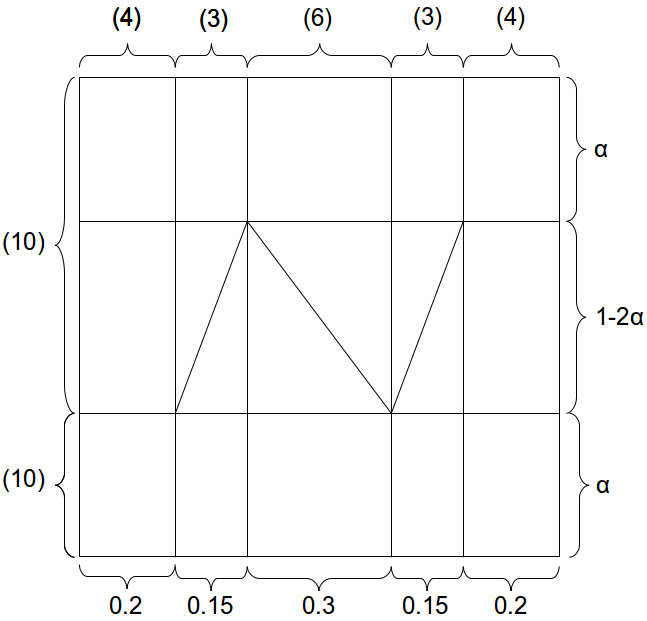
\includegraphics[width=5cm]{z_mesh}
  \caption{Z-mesh ((x) is the number of divisions and Y is the distance in cm)}
  \label{fig_z_mesh}
\end{figure}    
We compare the solution of the diffusion equation using the Z-mesh
\Cref{z_mesh_sol} with $\alpha=0.2$ with the one obtained using an uniform \Cref{u_mesh_sol}. 
The domain is 1cm by 1cm and is discretized using 20 by 20 cells. All the 
boundary conditions are vacuum. The medium is homogeneous $\Sigma_a = 0.5 cm^{-1}$ 
and $D=2$. There is a uniform source of intensity 1.                  
\begin{figure}[H]
  \centering
  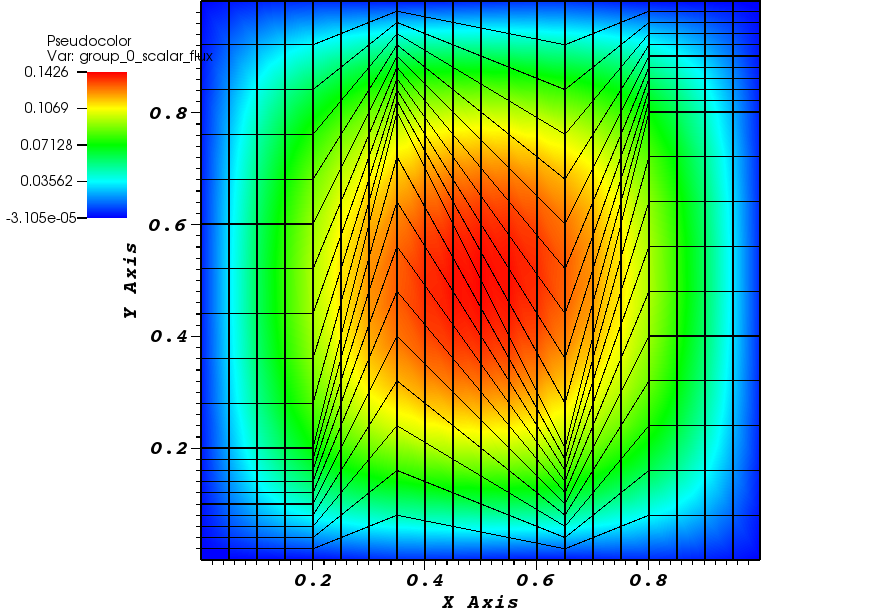
\includegraphics[width=5cm]{z_mesh_sol}
  \caption{Scalar flux on the z-mesh}
  \label{z_mesh_sol}
\end{figure}
\begin{figure}[H]
  \centering
  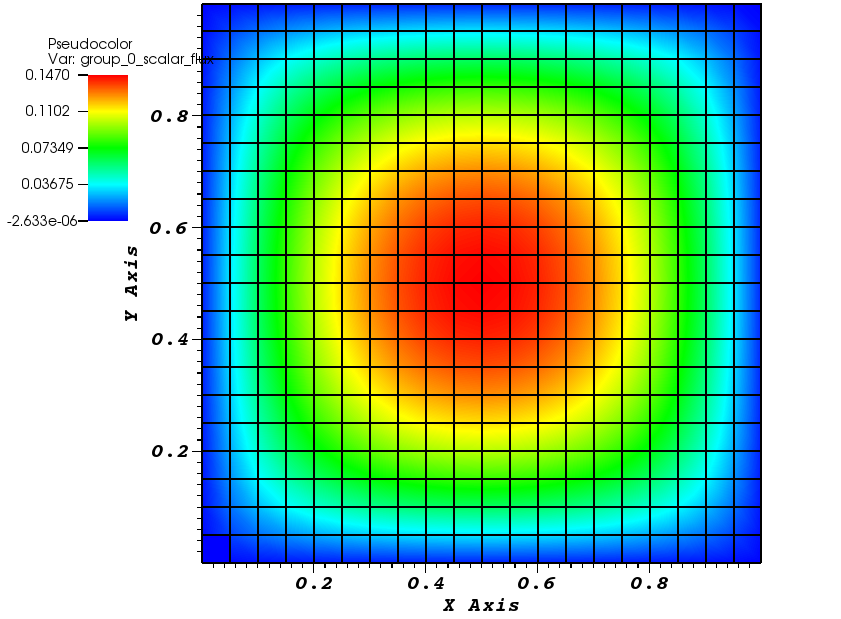
\includegraphics[width=5cm]{pwld_uniform_sol}
  \caption{Scalar flux on the uniform mesh}
  \label{u_mesh_sol}
\end{figure}
\subsection{Randomized polygonal grid}
\subsection{AMR}
The AMR problem is composed of two regions, see \Cref{amr_regions}.
\begin{figure}[H]
  \centering
  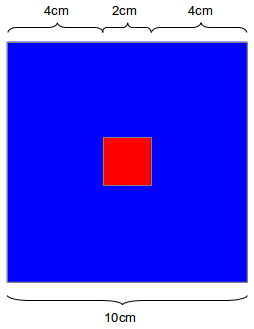
\includegraphics[width=3cm]{amr_zones}
  \caption{Regions of the AMR problem.}
  \label{amr_regions}
\end{figure}
The domain is a square of 10cm side (blue region) with in its center a smaller
square of 2cm side (red region). In the blue region, we have
$\Sigma_t=2cm^{-1}$ and $\Sigma_s=1cm^{-1}$. In the red region, we have
$\Sigma_t=1cm^{-1}$, $\Sigma_s=0.8cm^{-1}$, and a source of intensity $10
n/cm^{2}$. We use vacuum boundaries. The domain is initially discretize using
an uniform mesh of five by five cells. This mesh is then refined three
times. For each refinement, the cells with an estimated error of 70\% or more
of the largest estimated error are refined.
